\documentclass[12pt,a4paper]{article}
\usepackage{solutions-en}
\usepackage{float}

\title{Homework of 10.12\\Differential equations and dynamic systems.\\Solutions.}
\author{Глеб Минаев @ 204 (20.Б04-мкн)}
\date{}

\begin{document}
    \maketitle

    \begin{problem}{214}
        \begin{gather*}
            (x^2 - \sin(y)^2)dx + x \sin(2y) dy = 0\\
        \end{gather*}
        Let $f = x^2 - \sin(y)^2$, $g = x \sin(2y)$. Try to find function $\mu(x)$ such that
        \begin{gather*}
            \frac{\partial(f\mu)}{\partial y} = \frac{\partial(g\mu)}{\partial x}\\
            \frac{\partial f}{\partial y} \mu = \frac{\partial g}{\partial x} \mu + \frac{\partial \mu}{\partial x} g\\
            \left(\frac{\partial f}{\partial y} - \frac{\partial g}{\partial x}\right) \mu = g \mu'\\
            \mu = C e^{\int_{x_0}^x \frac{\frac{\partial f}{\partial y}(t) - \frac{\partial g}{\partial x}(t)}{g(t)} dt} = C e^{\int_{x_0}^x \frac{- \sin(2y) - \sin(2y)}{t \sin(2y)} dt} = Ce^{\int_1^x \frac{-2}{t} dt} = C x^{-2} = x^{-2}.
        \end{gather*}
        Hence
        \begin{align*}
            U(x, y)
            &:= \int_{x_0}^x (f\mu)(t, y_0) dt + \int_{y_0}^y (g\mu)(x, t) dt\\
            &= \int_{x_0}^x \left(1 - \frac{\sin(y_0)^2}{t^2}\right) dt + \int_{y_0}^y \frac{\sin(2t)}{x} dt\\
            &= \left.\left(t + \frac{\sin(y_0)^2}{t}\right)\right|_{x_0}^x + \left.\frac{-\cos(2t)}{2x}\right|_{y_0}^{y}\\
            &= x - x_0 - \frac{1 - \cos(2y_0)}{2x_0} + \frac{1 - \cos(2y_0)}{2x} + \frac{-\cos(2y)}{2x} - \frac{-\cos(2y_0)}{2x}\\
            &= x - x_0 - \frac{1 - \cos(2y_0)}{2x_0} + \frac{1}{2x} + \frac{-\cos(2y)}{2x}\\
            &= x - x_0 - \frac{\sin(y_0)^2}{x_0} + \frac{\sin(y)^2}{x}\\
            &= x + \frac{\sin(y)^2}{x}
        \end{align*}
        is integral of the equation. Hence
        \begin{gather*}
            x + \frac{\sin(y)^2}{x} = C\\
            \sin(y)^2 = Cx - x^2\\
            y = \sin^{-1}(\sqrt{Cx - x^2}).
        \end{gather*}
    \end{problem}

    \begin{problem}{215}
        \begin{gather*}
            x(\ln(y) + 2\ln(x) - 1)dy = 2y dx\\
            2y dx + x(1 - \ln(y) - 2\ln(x))dy = 0
        \end{gather*}
        Let $f = 2y$, $g = x(1 - \ln(y) - 2\ln(x))$. Try to find function $\mu(x, y)$ such that
        \begin{gather*}
            \frac{\partial(f\mu)}{\partial y} = \frac{\partial(g\mu)}{\partial x}\\
            \frac{\partial f}{\partial y} \mu + \frac{\partial \mu}{\partial y} f = \frac{\partial g}{\partial x} \mu + \frac{\partial \mu}{\partial x} g\\
            \left(\frac{\partial f}{\partial y} - \frac{\partial g}{\partial x}\right) \mu + \frac{\partial \mu}{\partial y} f - \frac{\partial \mu}{\partial x} g = 0
        \end{gather*}
        Let's consider $\mu$ as composition $\sigma \circ \eta$ for some $\sigma(t)$, $\eta(x, y)$. So
        \begin{gather*}
            \left(\frac{\partial f}{\partial y} - \frac{\partial g}{\partial x}\right) \sigma(\eta) + \left(\frac{\partial \eta}{\partial y} f - \frac{\partial \eta}{\partial x} g\right) \sigma'(\eta) = 0\\
            (\ln(\sigma))'(\eta) = \frac{\sigma'(\eta)}{\sigma(\eta)} = \frac{\frac{\partial f}{\partial y} - \frac{\partial g}{\partial x}}{\frac{\partial \eta}{\partial x} g - \frac{\partial \eta}{\partial y} f}
        \end{gather*}
        In terms of current $f$ and $g$
        \[
            (\ln(\sigma))'(\eta) = \frac{3 + 2\ln(x) + \ln(y)}{\frac{\partial \eta}{\partial x} x(1 - 2\ln(x) - \ln(y)) - \frac{\partial \eta}{\partial y} 2y}
        \]
        Let $\eta = x y^2$. So $\frac{\partial \eta}{\partial x} = \eta/x$, $\frac{\partial \eta}{\partial y} = 2\eta/y$,
        \begin{align*}
            (\ln(\sigma))'(\eta)
            &= \frac{3 + 2\ln(x) + \ln(y)}{\eta(1 - 2\ln(x) - \ln(y)) - 4\eta}\\
            &= \frac{3 + 2\ln(x) + \ln(y)}{\eta(-3 - 2\ln(x) - \ln(y))}\\
            &= \frac{-1}{\eta}
        \end{align*}
        \begin{gather*}
            \ln(\mu) = \ln(\sigma(\eta)) = - \ln(\eta)\\
            \mu = \frac{1}{x y^2}\\
        \end{gather*}
        Hence
        \begin{align*}
            U(x, y)
            &:= \int_{x_0}^x (f\mu)(t, y_0) dt + \int_{y_0}^y (g\mu)(x, t) dt\\
            &= \int_{x_0}^x \frac{2}{t y_0} dt + \int_{y_0}^y \frac{1 - \ln(t) - 2\ln(x)}{t^2} dt\\
            &= \left.\frac{2}{y_0} \ln(t)\right|_{x_0}^x + \left.\frac{2 \ln(x) + \ln(y)}{y}\right|_{y_0}^y\\
            &= -\frac{2\ln(x_0)}{y_0} + \frac{2 \ln(x) + \ln(y) - \ln(y_0)}{y}\\
            &= \frac{2 \ln(x) + \ln(y)}{y}\\
        \end{align*}
        is integral of the equation. Hence
        \begin{gather*}
            \frac{2 \ln(x) + \ln(y)}{y} = C\\
            Cy = \ln(x^2 y)
        \end{gather*}
        which solutions is not elemantary functions.
    \end{problem}

    \begin{problem}{242}
        \begin{gather*}
            8(y')^3 = 27 y\\
            2y' = 3 \sqrt[3]{y}\\
            \intertext{(dividing by $\sqrt[3]{y}$ lose solution $y \equiv 0$)}
            \frac{2}{3} \frac{y'}{y^{1/3}} = 1\\
            (y^{2/3})' = 1\\
            y^{2/3} = C + x\\
            y = \pm (C + x)^{3/2}.
        \end{gather*}
        It's easy to see that any point $(x_0; y_0)$ where $y_0 \neq 0$ is a point of uniqness, because it's not solution of $y \equiv 0$, so it can be a solution of only $y = \pm (C + x)^{3/2}$, then $C = y_0^{2/3} - x_0$ and sign in the formula is determined by sign of $y_0$, so the solution is realy unique. But any point $(x_0; 0)$ is not a point of uniqness, because there are three different solutions $y \equiv 0$, $y = (x - x_0)^{3/2}$ and $y = -(x - x_0)^{3/2}$. Hence $y \equiv 0$ is only singular solution.
        \begin{figure}[H]
            \centering
            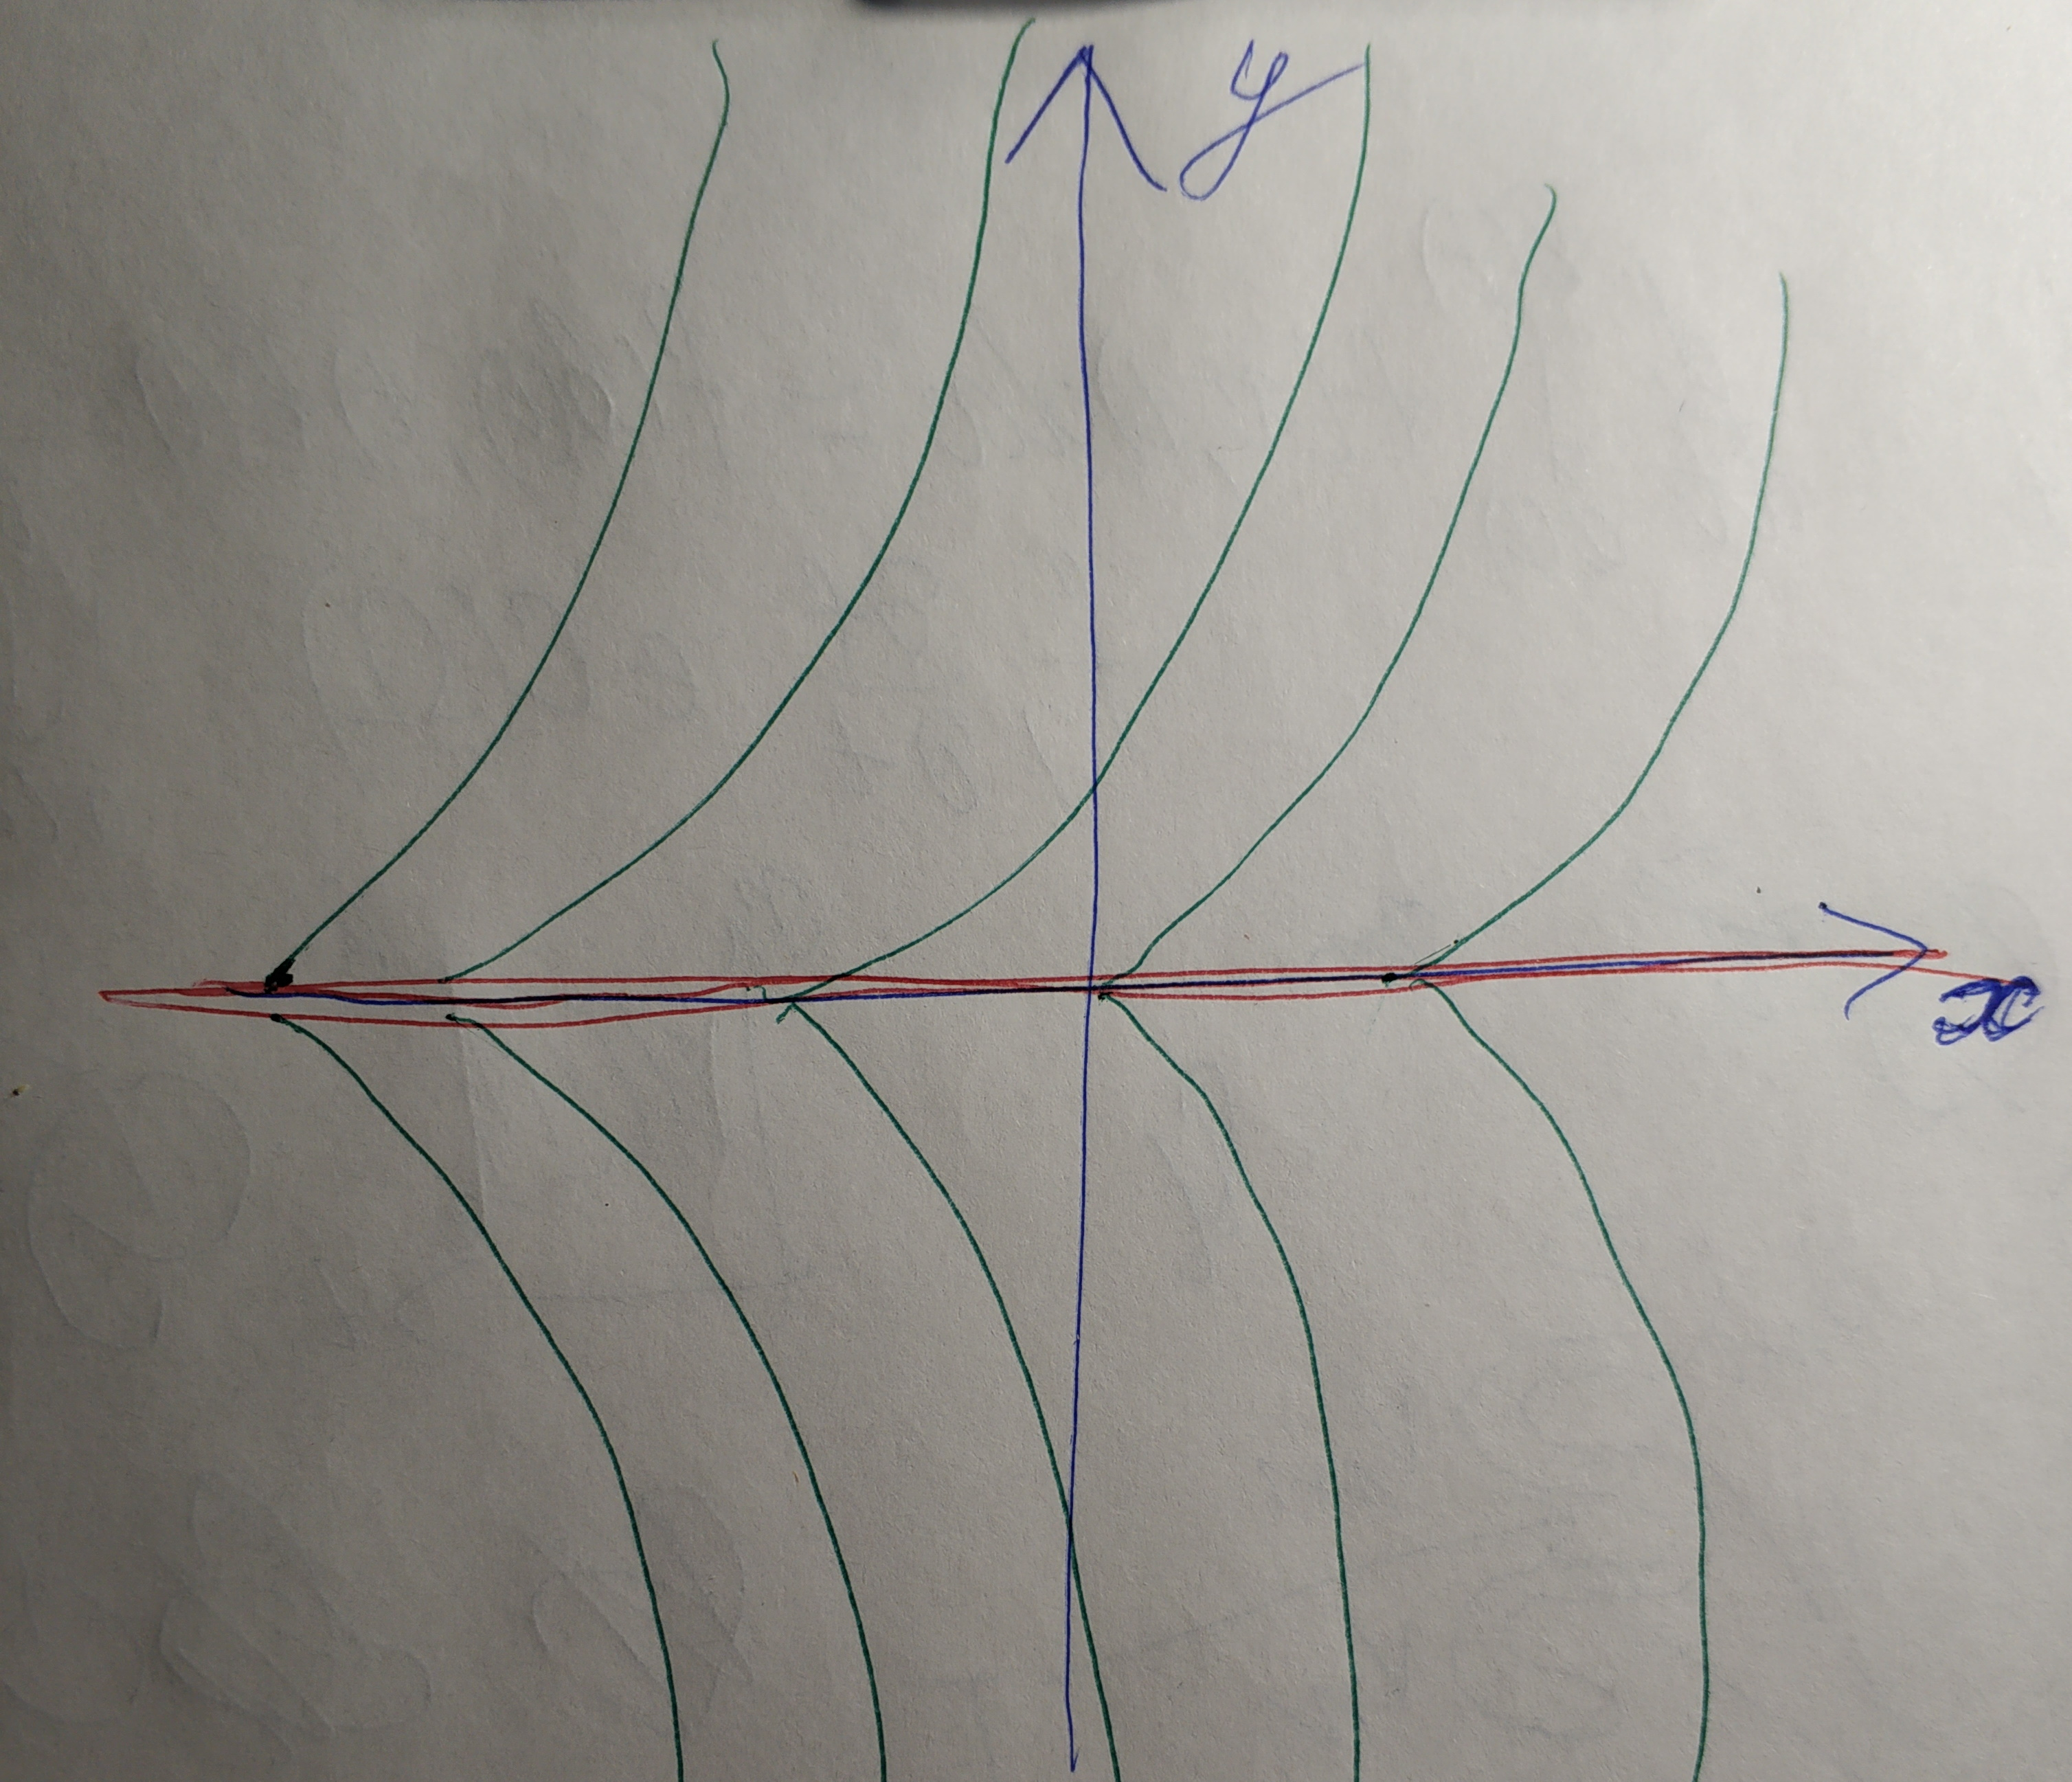
\includegraphics[height=7cm]{DEaDS-HW-006.jpg}
            \caption{Red line --- singular solution, green lines --- samples of other solution.}
        \end{figure}
    \end{problem}
\end{document}